% Adjust these for the path of the theme and its graphics, relative to this file
%\usepackage{beamerthemeFalmouthGamesAcademy}
\usepackage{../../beamerthemeFalmouthGamesAcademy}
\usepackage{multimedia}
\usepackage{soul}
\usepackage{tikz}
\usepackage{enumitem}
\usepackage{verbatim}
\graphicspath{ {../../} }

% Default language for code listings
\lstset{language=C++,
        morekeywords={each,in,nullptr}
}

% For strikethrough effect
\usepackage[normalem]{ulem}
\usepackage{wasysym}

\usepackage{pdfpages}

% http://www.texample.net/tikz/examples/state-machine/
\usetikzlibrary{arrows,automata}

\newcommand{\modulecode}{COMP260}\newcommand{\moduletitle}{Distributed Systems}\newcommand{\sessionnumber}{5}

\def\signed #1{{\leavevmode\unskip\nobreak\hfil\penalty50\hskip2em
  \hbox{}\nobreak\hfil(#1)%
  \parfillskip=0pt \finalhyphendemerits=0 \endgraf}}

\newsavebox\mybox
\newenvironment{aquote}[1]
  {\savebox\mybox{#1}\begin{quote}}
  {\signed{\usebox\mybox}\end{quote}}

\newlist{todolist}{itemize}{2}
\setlist[todolist]{label=$\square$}

\begin{document}
\title{\sessionnumber: \normalsize{Human-Centred Design for AR/VR}}
\subtitle{\modulecode: \moduletitle}

\frame{\titlepage} 
% LEARNING OUTCOMES
\begin{frame}
	\frametitle{Virtual and Augmented Reality Overview:}
	
	\textbf{Learning Outcomes:}
	
	\begin{itemize}
		\item \textbf{Explain} the difference between augmented \& virtual reality. 
		\item \textbf{Discuss} the various forms of haptic feedback.
		\item \textbf{List} and \textbf{describe} the key components that make up the hardware side of reality systems.	
	\end{itemize}
\end{frame}

\begin{frame}
	\frametitle{Personal Brand}
	\begin{figure}
		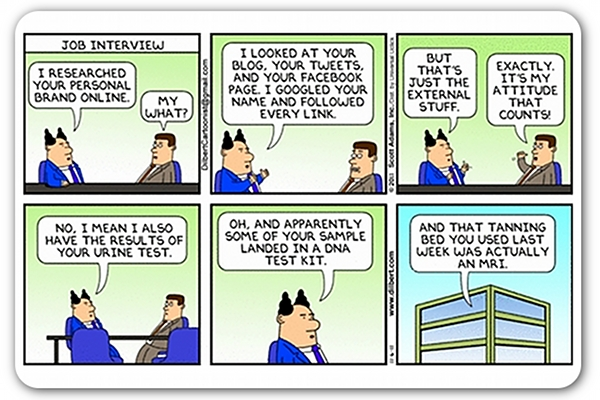
\includegraphics[scale=.5]{assets/personal-brand}
	\end{figure}
\end{frame}

%what

\begin{frame}
	\begin{figure}
		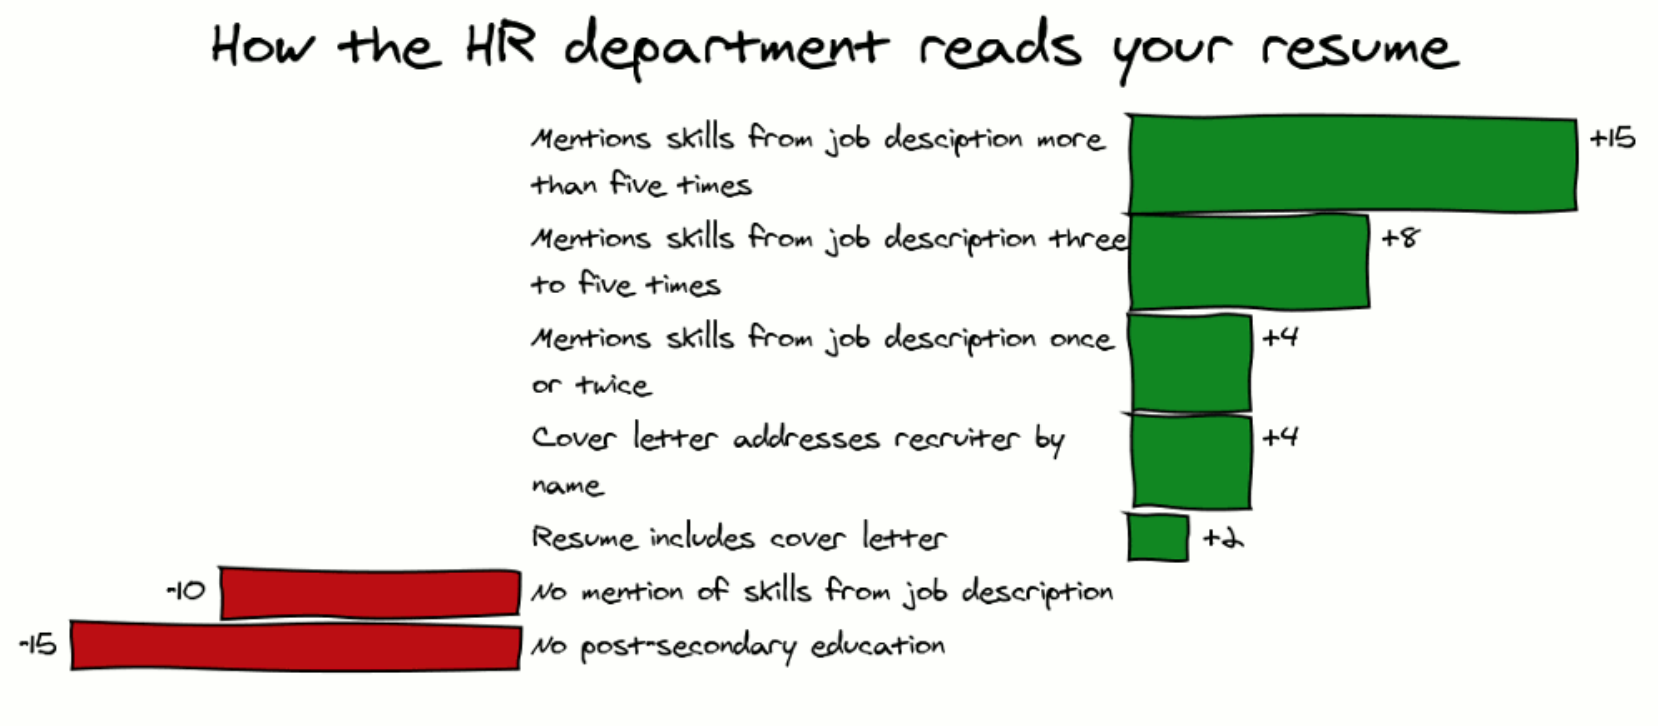
\includegraphics[scale=.35]{assets/diff1}
	\end{figure}
\end{frame}

\begin{frame}
	\begin{figure}
		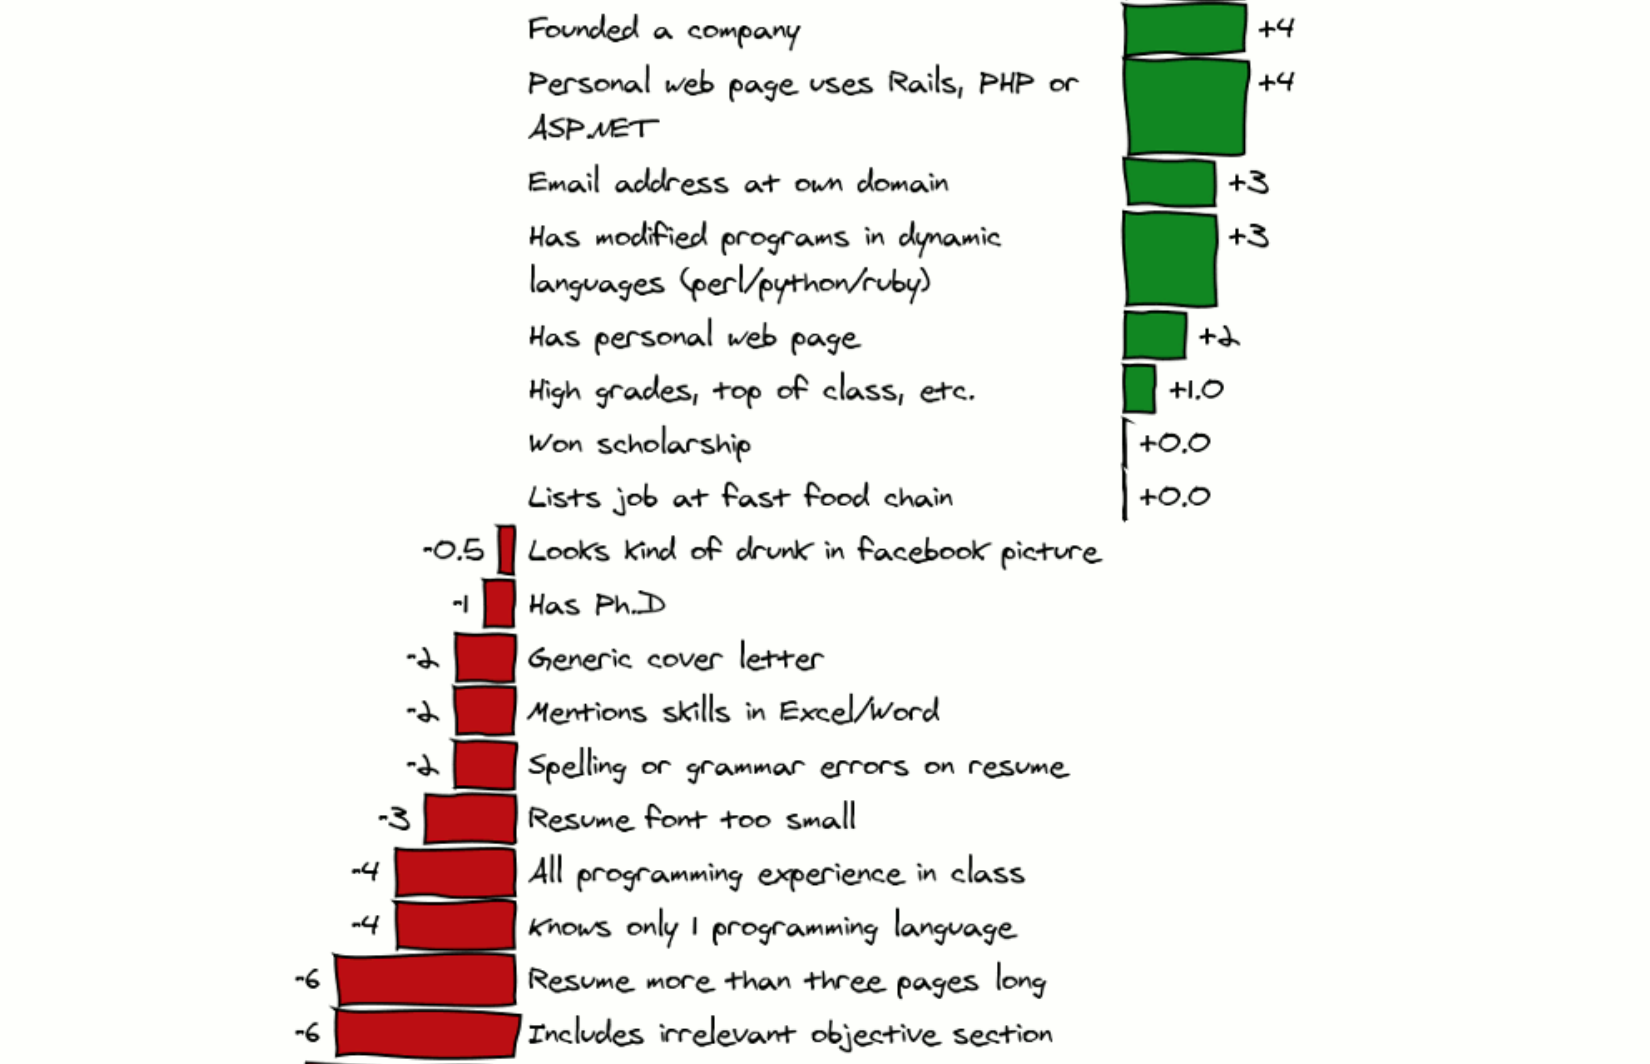
\includegraphics[scale=.35]{assets/diff2}
	\end{figure}
\end{frame}

\begin{frame}
	\begin{figure}
		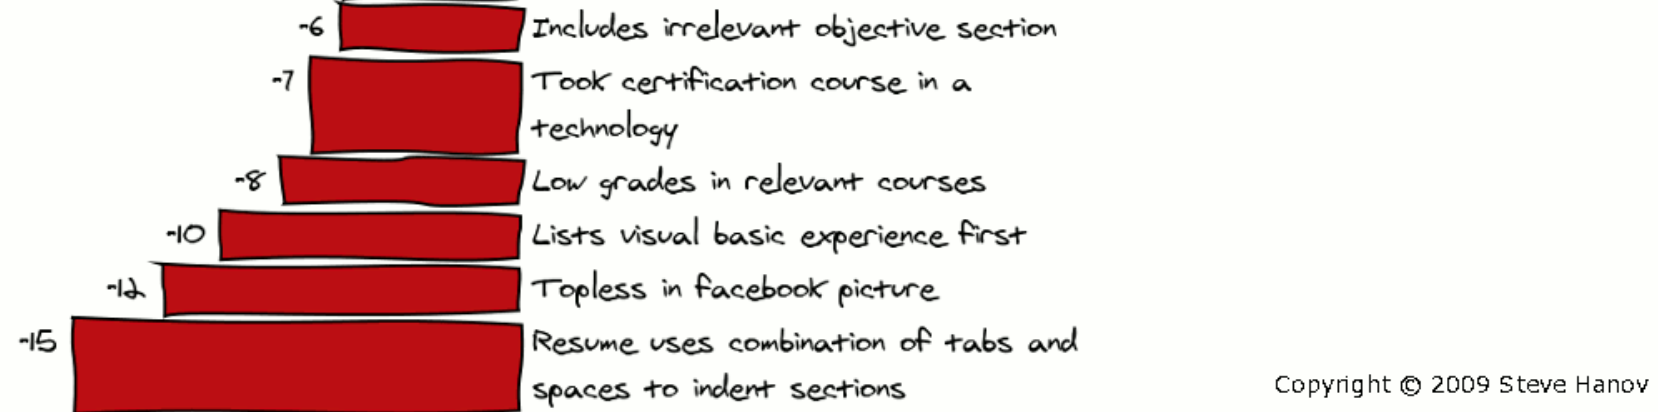
\includegraphics[scale=.35]{assets/diff3}
	\end{figure}
\end{frame}

\begin{frame}
	\begin{figure}
		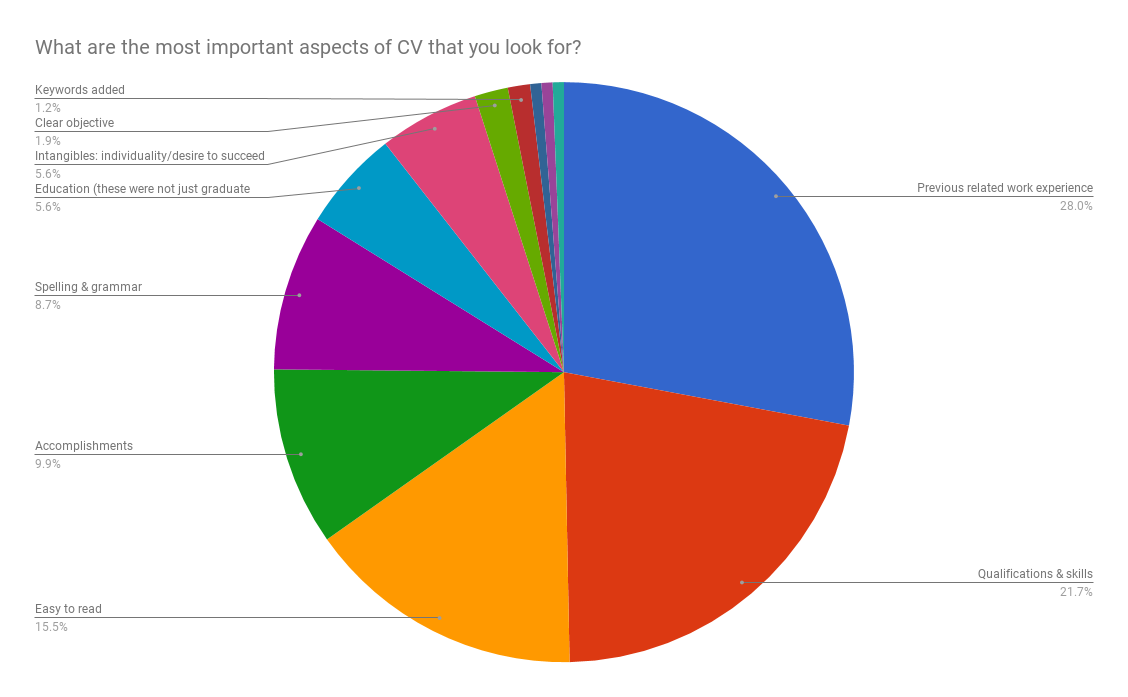
\includegraphics[scale=.27]{assets/priority}
		\caption{2010 Employers Survey}
	\end{figure}
	\href{http://stevehanov.ca/blog/resume_comic.png}{source}
\end{frame}

\begin{frame}
	\begin{figure}
		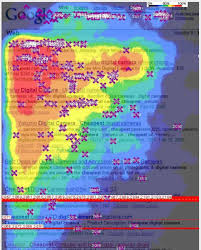
\includegraphics[scale=.8]{assets/golden-triangle}
		
	\end{figure}
	\href{www.forbes.com/sites/roberthof/2015/03/03/how-do-you-google-new-eye-tracking-study-reveals-huge-changes/\#604c90423828}{source}
\end{frame}

\begin{frame}
	\frametitle{No One Size Fits All}
	\begin{figure}
		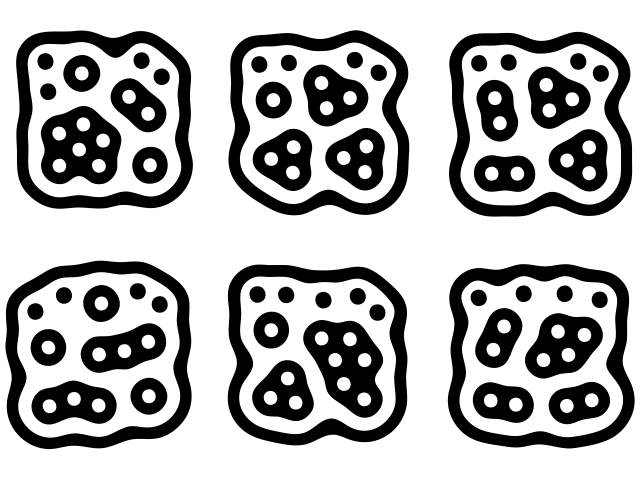
\includegraphics[scale=.5]{assets/reactivision}
	\end{figure}
\end{frame}



\begin{frame}
	\frametitle{When?}
	\pause fluid document
	\pause Grows with you
	\pause Becomes more tailored to you career 
	\pause More you! 
	
\end{frame}

%CONTENT

\begin{frame}
	\frametitle{Personal Details}
	
	\begin{itemize}
		\item Name (Obviously)
		\item Address
		\item Telephone Numbers
		\item Email
		\item Website Address (Portfolio)
	\end{itemize}

	\pause
	You are not required to provide any further information. 
	\begin{itemize}
		\item Age
		\item Gender
		\item Nationality
		\item ... 
	\end{itemize}

\end{frame}

\begin{frame}
	\frametitle{No Rockstar Profile Pic}
	\begin{figure}
		
\includegraphics[scale=.3]{assets/rockstar}
	\end{figure}
\end{frame}

\begin{frame}
	\frametitle{No Rockstar Email}
	\begin{figure}
		
\includegraphics[scale=.3]{assets/email}
	\end{figure}
\end{frame}

\begin{frame}
	\frametitle{Profile (optional)}
	\begin{itemize}
		\item \st{Optional} Encouraged 
		\item Three to four lines length
		\item STRESSFUL - Important to get right
		\item Omit if unsure
	\end{itemize}
\end{frame}

\begin{frame} 
	\frametitle{Qualifications}
	\begin{itemize}
		\item Reverse chronological order
		\item Current course listed at top
		\item Provide more info for most recent/relevant qualifications - it is helpful to name the various modules of your degree. 
	\end{itemize}
\end{frame}

\begin{frame}
	\begin{aquote}{Creative CV Guide - Jan Cole}
	Additional relevant information about your degree may be included in this section, elsewhere in your CV or in
your accompanying email or letter. This could include details of modules studied to emphasise the nature of
your degree, the subject of your dissertation to show a particular area of interest, or details of live projects to
demonstrate commercial experience. 
  	\end{aquote}
	\begin{figure}
	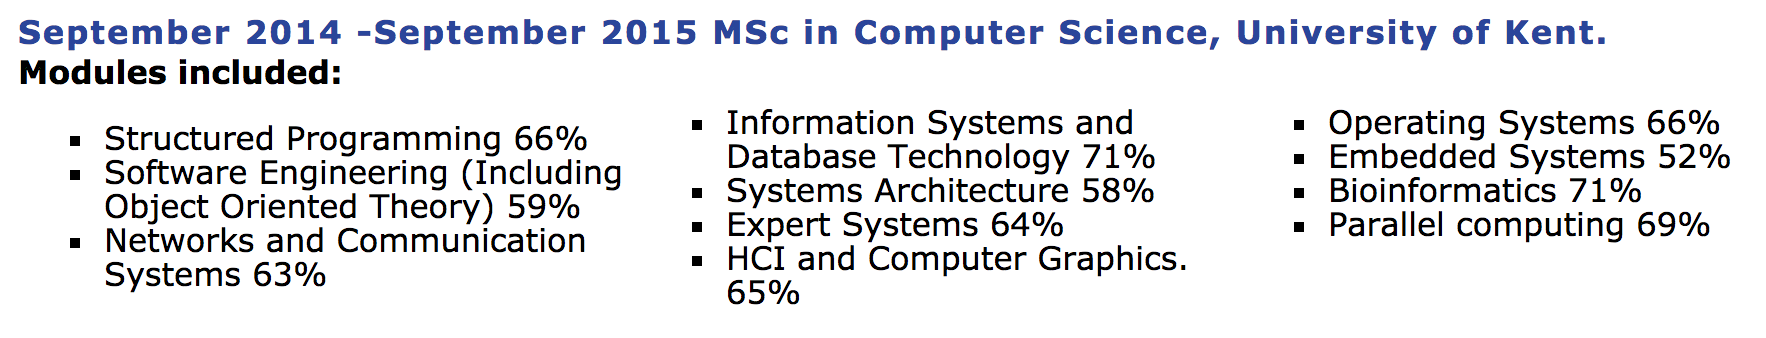
\includegraphics[scale=.3]{assets/qual}
	\end{figure}
\end{frame}

\begin{frame} 
	\frametitle{Experience}
	\begin{itemize}
	 	\item Start and end dates
	 	\item Name of organisation
		\item Position or role
	 	\item Brief outline of responsibilities \& achievements (try not to repeat yourself!)
		\item RC order!
	\end{itemize}	
\end{frame}

\begin{frame} 
	\frametitle{Skills}
	\begin{itemize}
	 	\item Group skills into appropriate categories (Computer Skills, Communication Skills, Project management...)
	 	\item Keep them relevant 
	 	\item Brief outline of responsibilities \& achievements (try not to repeat yourself!)
		\item RC order!
	\end{itemize}	
\end{frame}

\begin{frame}
	TECHNICAL SKILLS (Example)
	\begin{itemize}
		\item \textbf{SECURITY: }McAfee SIEM/EPO/NSM, FireEye CMS/ETP, SecureWorks, IDS/IPS, Sumo Logic cloud-based log management, SSL certificate configuration and management, Juniper NetScreen/Palo Alto Networks firewall
		\item \textbf{REVERSE ENGINEERING: } Ollydbg, WinBdg, GBD, IDA Pro, PEiD, malware sandbox
		\item \textbf{NETWORKING: } Wireshark/TCPView packet analysis, DNS servers, mail server
		\item \textbf{OPERATING SYSTEMS:} Windows XP, Vista, 7, 8; Windows Server 2003, 2008, 2012; Linux including CentOS, Ubuntu, Arch, Debian, BackTrack, and Kali
	\end{itemize}
\end{frame}

\begin{frame}
	\frametitle{Other}
	
	\begin{itemize}
		\item Training \& short courses (Those that do not constitute a qualification)
		\item Addition information \pause
		\begin{itemize}
			\item scholarships, sponsorship, awards, responsibilities, competitions, other languages, public speaking, teaching experience...
		\end{itemize}
		\item Interests \& activities
		\begin{itemize}
			\item These must be relevant to the career opportunity.
		\end{itemize}
	\end{itemize}
\end{frame}

\begin{frame}
	\frametitle{ To Ref or Not To Ref?}
	
	Should you include references?
	\pause
	
	if you are sending out CVs unsolicited just include the phrase `references available on request' somewhere in the document.
	
	\pause
	
	If the CV has been requested then the employer will probably ask you to include two references.
	
\end{frame}

% MORE TIPS 
\begin{frame}
\frametitle{ACTION WORDS}
\begin{columns}
	\begin{column}{0.3\textwidth}
Planned	Devised	Achieved
Developed	Liaised (spell it right!)	Evaluated
Supervised	Co-ordinated	Managed
Administered	Controlled	 Selected
	\end{column}
	\begin{column}{0.3\textwidth}  
Designed	Researched	Analysed
Discovered	Recommended	Tested
Diagnosed	Budgeted	Monitored
Evaluated	
	\end{column}
	\begin{column}{0.3\textwidth}   
Selected	Trained	Taught
Explained	Presented	Conducted
Distributed	Organised	Solved
Represented	Persuaded	Calculated	
	\end{column}
\end{columns}
\vspace{1cm}
\href{https://www.kent.ac.uk/careers/cv/actionverbs.htm}{SOURCE}

\end{frame}

\begin{frame}
	\frametitle{Check Lists}
	\begin{itemize}
		\item Content:
  		\begin{todolist}
			\item Ensure your profile clearly shows that you have the key qualities for the job.
    			\item Present the information clearly and concisely.
			\item Place sections that contain your strongest qualities before less impressive information.
			\item Write your CV in the third person. Avoid using ?I? or referring to yourself by name.
			\item Check that you have not repeated information or included anything that is not relevant.
			\item Use correct industry terminology
    		 \end{todolist}
	\end{itemize}
\end{frame}

\begin{frame}
	\frametitle{Check Lists}
	\begin{itemize}
		\item Presentationt:
  		\begin{todolist}
			\item Scrutinise your CV for spacing and layout inconsistencies.
			\item Choose a clear, attractive format that is appropriate for the organisation.
			\item Ensure the balance between text, images and white space are pleasing to the eye.
			\item Give careful consideration to the style, size and colour of font.
			\item If your CV is multiple pages, ensure there is consistency between them.
    		 \end{todolist}
	\end{itemize}
	Source - Creative CV Guide - Jan Cole
\end{frame}

\begin{frame}
	Your turn!
\end{frame}

\begin{frame}
	\frametitle{Further Learning}
\end{frame}


\end{document}
